\documentclass{beamer}
\usepackage[utf8]{inputenc}
\usetheme{Copenhagen}
\usepackage{color}
\usepackage{amsmath}
\usepackage{amsthm}
\usepackage{listings}
\usepackage{graphicx}
\usepackage{braket}

\newtheorem{thm}{Theorem}

\title{Cracking RSA with Quantum Computing}
\author{Max Ovsiankin}
\date{May 9, 2018}

\begin{document}

\begin{frame}
    \titlepage
\end{frame}

\begin{frame}
    \frametitle{Outline}
    \tableofcontents
\end{frame}
\section{The Setting}

\begin{frame}{The Setting}
    RSA is a commonly used set of algorithms that provides security when sending encrypted messages. \pause 
    
    Crucially, the security of RSA depends on the hardness of factoring a number $N = pq$, where $p$ and $q$ are large prime numbers ('secrecy'). \pause

\end{frame}

\begin{frame}{The Setting}
    An assumption of RSA security (that follows from $\textsc{P} \neq \textsc{NP}$) is that prime numbers cannot be factored with a polynomial-time algorithm in the number of bits of $N$. \pause
    
    Quantum computers \textit{are} able to factor in polynomial time. This talk will focus on explaining how quantum algorithms work, building up to Shor's famous algorithm for factoring.
\end{frame}

\section{Classical Computers}
\begin{frame}{What Computers Look Like}
Equivalent to a circuit whose representation can be quickly computed: \\
\ \\

\centering 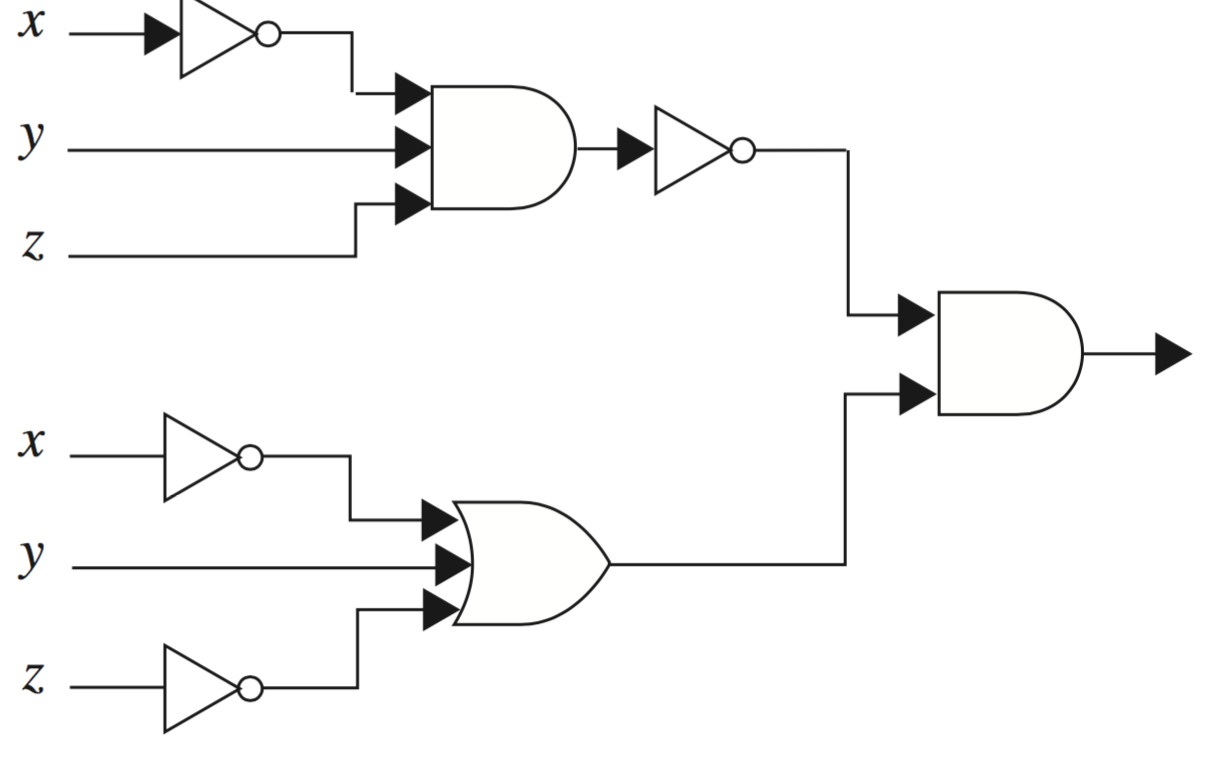
\includegraphics[height=4cm]{bool-circuit.png}
\end{frame}
\begin{frame}{What Computers Look Like}
We can think of a circuit as having $n$ registers, each of which contain 0 or 1.
A possible \textit{state} of these $n$ registers is an element of $\{ 0, 1 \}^n$ (n-length bitstring).
Then the action of a gate can be described as a matrix of 0s and 1s.
\end{frame}
\begin{frame}{What Computers Look Like: NOT gate}
    \textsc{NOT} gate:
    
    $$ \textsc{NOT}(0) = 1$$
    $$ \textsc{NOT}(1) = 0$$
    
    \ \\
    
    \pause Let's relabel $0 = \begin{bmatrix}
        1 \\
        0
    \end{bmatrix}$, $1 = \begin{bmatrix}
        0 \\
        1
    \end{bmatrix}$.
    
    Elements of a 2-element vector space, as there are 2 possibilities for bits.
\end{frame}
\begin{frame}{What Computers Look Like: NOT gate}
    \textsc{NOT} gate:
    
    $$ \textsc{NOT}\left(\begin{bmatrix}
        1 \\
        0
    \end{bmatrix}\right) = \begin{bmatrix}
        0 \\
        1
    \end{bmatrix}$$
    $$ \textsc{NOT}\left(\begin{bmatrix}
        0 \\
        1
    \end{bmatrix}\right) = \begin{bmatrix}
        1 \\
        0
    \end{bmatrix}$$
    
    This strongly suggests we can consider it as a matrix: $$\textsc{NOT} = \begin{bmatrix}
        0 & 1 \\
        1 & 0 \\
    \end{bmatrix}$$
\end{frame}
\begin{frame}{What Computers Look Like: AND gate}
    \textsc{AND} gate:
    
    $$ \textsc{AND}\left(0, 0\right) = 0$$
    $$ \textsc{AND}\left(0, 1\right) = 0$$
    $$ \textsc{AND}\left(1, 0\right) = 0$$
    $$ \textsc{AND}\left(1, 1\right) = 1$$
\end{frame}
\begin{frame}{What Computers Look Like: AND gate}
    For two input bits, there are $4 = 2^2$ possible states. 
    
    $$ (0, 0) = \ket{00} = \ket{0} \otimes \ket{0}$$
    $$ (0, 1) = \ket{01} = \ket{0} \otimes \ket{1}$$
    $$ (1, 0) = \ket{10} = \ket{1} \otimes \ket{0}$$
    $$ (0, 1) = \ket{11} = \ket{1} \otimes \ket{1}$$
\end{frame}
\begin{frame}{What Computers Look Like: AND gate}
    $$ \textsc{AND}\left(\ket{00}\right) = \ket{0}$$
    $$ \textsc{AND}\left(\ket{01}\right) = \ket{0}$$
    $$ \textsc{AND}\left(\ket{10}\right) = \ket{0}$$
    $$ \textsc{AND}\left(\ket{11}\right) = \ket{1}$$
\end{frame}
\begin{frame}{What Computers Look Like: AND gate}
    $$ \textsc{AND}\left(1\ket{00}+0\ket{01}+0\ket{10}+0\ket{11}\right) = 1\ket{0}+0\ket{1}$$
    $$ \textsc{AND}\left(0\ket{00}+1\ket{01}+0\ket{10}+0\ket{11}\right) = 1\ket{0}+0\ket{1}$$
    $$ \textsc{AND}\left(0\ket{00}+0\ket{01}+1\ket{10}+0\ket{11}\right) = 1\ket{0}+0\ket{1}$$
    $$ \textsc{AND}\left(0\ket{00}+0\ket{01}+0\ket{10}+1\ket{11}\right) = 0\ket{0}+1\ket{1}$$
\end{frame}
\begin{frame}{What Computers Look Like: AND gate}
    
    $$ \begin{bmatrix}
        1 & 1 & 1 & 0 \\
        0 & 0 & 0 & 1
    \end{bmatrix}\left(1\ket{00}+0\ket{01}+0\ket{10}+0\ket{11}\right) = 1\ket{0}+0\ket{1}$$
    $$ \begin{bmatrix}
        1 & 1 & 1 & 0 \\
        0 & 0 & 0 & 1
    \end{bmatrix}\left(0\ket{00}+1\ket{01}+0\ket{10}+0\ket{11}\right) = 1\ket{0}+0\ket{1}$$
    $$ \begin{bmatrix}
        1 & 1 & 1 & 0 \\
        0 & 0 & 0 & 1
    \end{bmatrix}\left(0\ket{00}+0\ket{01}+1\ket{10}+0\ket{11}\right) = 1\ket{0}+0\ket{1}$$
    $$ \begin{bmatrix}
        1 & 1 & 1 & 0 \\
        0 & 0 & 0 & 1
    \end{bmatrix}\left(0\ket{00}+0\ket{01}+0\ket{10}+1\ket{11}\right) = 0\ket{0}+1\ket{1}$$
\end{frame}
\begin{frame}{What Computers Look Like: AND gate}
    Okay, we have a vector space now. What about linear combinations?
    
    $$\begin{bmatrix}
        1 & 1 & 1 & 0 \\
        0 & 0 & 0 & 1
    \end{bmatrix}\left(\frac{1}{2}\ket{00}+0\ket{01}+\frac{1}{4}\ket{10}+\frac{1}{4}\ket{11}\right) = \ ???$$
    
\end{frame}
\section{Quantum Computers}
\begin{frame}{What changes for Quantum?}
    The state of an $n$-bit classical computer is a vector in $\mathbb{R}^{2^n}$ with only one coefficient nonzero. (we already saw this in explaining classical computers) \pause
    
    \ \\
    The state of an $n$-\textit{qu}bit quantum computer is a vector in $\mathbb{C}^{2^n}$ that is normalized (this reflects the underlying quantum property of superposition): \[
        a_0 \ket{00} +  a_1 \ket{01} + a_2 \ket{10} + a_3 \ket{11}
    \]
    with $a_i \in \mathbb{C}$ and $\sum_{i=0}^{n-1} |a_i|^2 = 1$ (unit vectors)
\end{frame}
\begin{frame}{What changes for Quantum?}
    The operation we perform on a $n$-qubit `register' is to measure it. \pause
    \[
        a_0 \ket{00} +  a_1 \ket{01} + a_2 \ket{10} + a_3 \ket{11}
    \] \pause
    
    This produces $\ket{00}$ with probability $|a_0|^2$, $\ket{01}$ with probability $|a_1|^2$, etc.
\end{frame}
\begin{frame}{Quantum Gates}
    Our quantum gates now take unit complex vectors to unit complex vectors (they are exactly the \textit{unitary} matrices)! \pause
    
    \ \\
    
\begin{columns}
  \column{.33\textwidth}
   \centering Hadmard
   \[
   \frac{1}{\sqrt{2}}
   \begin{bmatrix}
   1 & 1  \\
   1 & -1
   \end{bmatrix}
   \] 
  \column{.33\textwidth}
   \pause \centering c-NOT
   \[
   \begin{bmatrix}
   1 & 0 & 0 & 0\\
   0 & 1 & 0 & 0\\
   0 & 0 & 0 & 1\\
   0 & 0 & 1 & 0
   \end{bmatrix}
   \]
  \column{.33\textwidth}
   \pause \centering Phase Rotation
   \[
   \begin{bmatrix}
   1 & 0 \\
   0 & e^{i \frac{\pi}{4}}
   \end{bmatrix}
   \]
\end{columns}
\end{frame}
\begin{frame}{Comparison to Classical}
    $$ \textsc{NOT}\left(1\ket{0}+0\ket{1}\right) = 0\ket{0}+1\ket{1}$$
    $$ \textsc{NOT}\left(0\ket{0}+1\ket{1}\right) = 1\ket{0}+0\ket{1}$$
\end{frame}
\begin{frame}{Comparison to Classical}
    $$ \begin{bmatrix}
        0 & 1 \\
        1 & 0
    \end{bmatrix} \left(1\ket{0}+0\ket{1}\right) = 1\ket{0}+0\ket{1}$$
    $$ \begin{bmatrix}
        0 & 1 \\
        1 & 0
    \end{bmatrix}\left(0\ket{0}+1\ket{1}\right) = 0\ket{0}+1\ket{1}$$
\end{frame}
\begin{frame}{Comparison to Classical}
    Superposition!
    
    $$ \begin{bmatrix}
        0 & 1 \\
        1 & 0
    \end{bmatrix}\left(\frac{1}{\sqrt{2}}\ket{0}+\frac{1}{\sqrt{2}}\ket{1}\right) = \frac{1}{\sqrt{2}}\left(\ket{0}+\ket{1}\right)$$
    
    Like applying the gate twice `at the same time'!
\end{frame}
\begin{frame}{c-NOT}
    Want a gate to `conditionally' apply its effect. Control bit controls whether gate act, and the gate acts on the second bit.
\end{frame}
\begin{frame}{c_NOT}
$$\begin{bmatrix}
   1 & 0 & 0 & 0\\
   0 & 1 & 0 & 0\\
   0 & 0 & 0 & 1\\
   0 & 0 & 1 & 0
   \end{bmatrix}(\ket{0} \otimes \ket{0}) = \ket{0} \otimes \ket{0}$$
   $$\begin{bmatrix}
   1 & 0 & 0 & 0\\
   0 & 1 & 0 & 0\\
   0 & 0 & 0 & 1\\
   0 & 0 & 1 & 0
   \end{bmatrix}(\ket{0} \otimes \ket{1}) = \ket{0} \otimes \ket{1}$$
\end{frame}
\begin{frame}{c_NOT}
$$\begin{bmatrix}
   1 & 0 & 0 & 0\\
   0 & 1 & 0 & 0\\
   0 & 0 & 0 & 1\\
   0 & 0 & 1 & 0
   \end{bmatrix}(\ket{1} \otimes \ket{0}) = \ket{1} \otimes \ket{1}$$
   $$\begin{bmatrix}
   1 & 0 & 0 & 0\\
   0 & 1 & 0 & 0\\
   0 & 0 & 0 & 1\\
   0 & 0 & 1 & 0
   \end{bmatrix}(\ket{1} \otimes \ket{1}) = \ket{1} \otimes \ket{0}$$
\end{frame}
\begin{frame}{Phase estimation}
    \textsc{Phase-estimate}
    
    \textbf{Input}: $\omega \in [0, 1]$ unknown. We get a state of the form $$
    \ket{\psi} = \frac{1}{\sqrt{2}^n} \sum_{i = 0}^{2^n - 1} e^{2 \pi i \omega y} \ket{y}$$
    \textbf{Output}: An estimate of $\omega$. \pause
    
    What does the output even look like? Need to approximate $\omega$ with $n$ bits when measured.
\end{frame} 
\begin{frame}{Phase estimation}

 \textsc{Phase-estimate}
 
    \textbf{Input}: $\omega \in [0, 1]$ unknown. We get a state of the form $$
    \ket{\psi} = \frac{1}{\sqrt{2}^n} \sum_{i = 0}^{2^n - 1} e^{2 \pi i \omega y} \ket{y}$$
    \textbf{Output}: An estimate of $\omega = 0.x_1 x_2 \ldots x_n = \frac{x}{2^n}$ for $x \in \{ 0, 1, 2, \ldots, 2^{n}-1\}$

\end{frame} 
\begin{frame}{Phase estimation}
    It turns out
    $$\frac{1}{\sqrt{2}^n} \sum_{i = 0}^{2^n - 1} e^{2 \pi i \omega y} \ket{y} = \frac{1}{\sqrt{2}^n} \left(\ket{0} + e^{2 \pi i 0.x_n} \ket{1} \right) \otimes \left(\ket{0} + e^{2 \pi i 0.x_{n-1} x_n} \ket{1} \right)$$
    $$\otimes \ldots  $$ 
    $$\otimes  \left(\ket{0} + e^{2 \pi i 0.x_{2} x_3 \ldots x_{n-1}} \ket{1} \right) \otimes \left(\ket{0} + e^{2 \pi i 0.x_{1} x_2 \ldots x_{n}} \ket{1} \right)$$ \pause
    
    Idea: `pull' $x_i$ out one by one, then remove them from the remaining bits.
\end{frame}
\begin{frame}{Phase estimation}
    Implementation (we will examine what happens):
    \centering 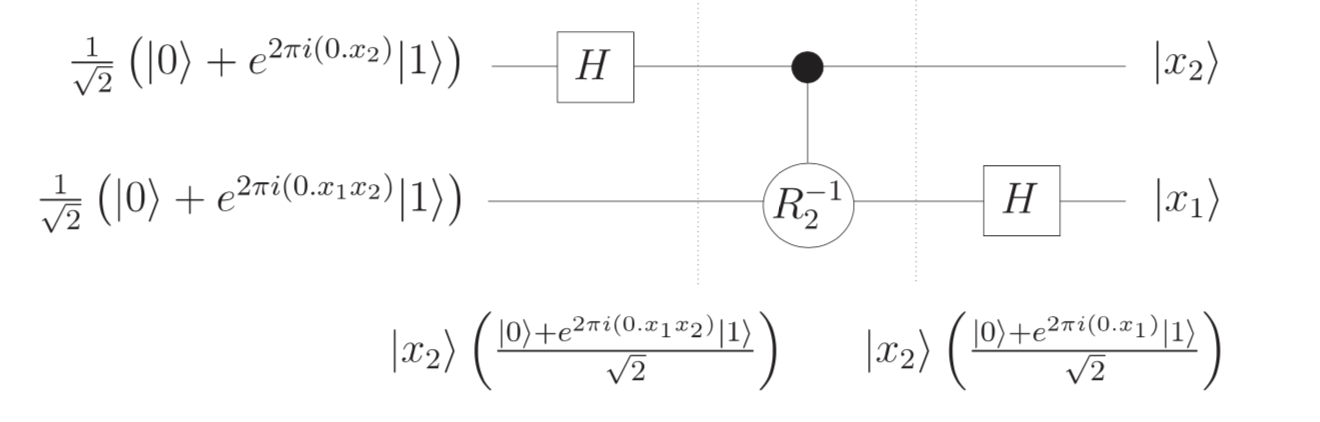
\includegraphics[height=3.5cm]{phase-estimation.png}
\end{frame}
\begin{frame}{Phase estimation}
    $$H = \frac{1}{\sqrt{2}} \begin{bmatrix}
        1 && 1 \\
        1 && -1
    \end{bmatrix}$$ 
    Looking at $$H \frac{1}{\sqrt{2}}(\ket{0} + e^{2\pi i (0.x_2)} \ket{1}) = H \frac{1}{\sqrt{2}}(\ket{0} + (-1)^{x_2} \ket{1}) = \ket{x_2}$$ \pause
    
    So $H$ `pulls' $x_2$ out for us, into a qbit!
\end{frame}
\begin{frame}{Phase estimation}
    We have $\ket{x_2}$ after the first $H$, and we want to `eliminate' it from the 2nd qubit:
    \centering 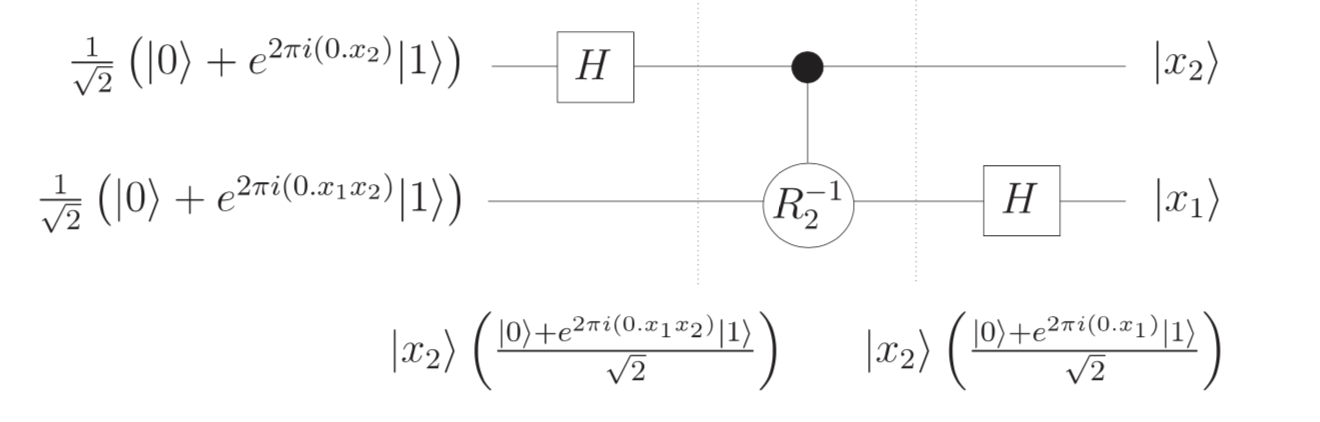
\includegraphics[height=3.5cm]{phase-estimation.png}
\end{frame}
\begin{frame}{Phase estimation}
    $$R_2^{-1} = \begin{bmatrix}
        1 & 0 \\
        0 & e^{- 2 \pi i (0.01)}
    \end{bmatrix}$$
    
    $R_2$ \textit{only} rotates the phase on $\ket{1}$.
    
    Action when $x_2 = 1$:
    
    $$R_2^{-1} \frac{1}{\sqrt{2}}(\ket{0} + e^{2\pi i (0.x_1 1)} \ket{1}) =  \frac{1}{\sqrt{2}}(\ket{0} + e^{2\pi i (0.x_1 0)} \ket{1})$$ \pause
    
    So we want to perform $R_2^{-1}$ only when $x_2 = 1$! So we use c-$R_2^{-1}$ instead.
\end{frame} 
\begin{frame}{Phase estimation}
    We are finished!
    \centering 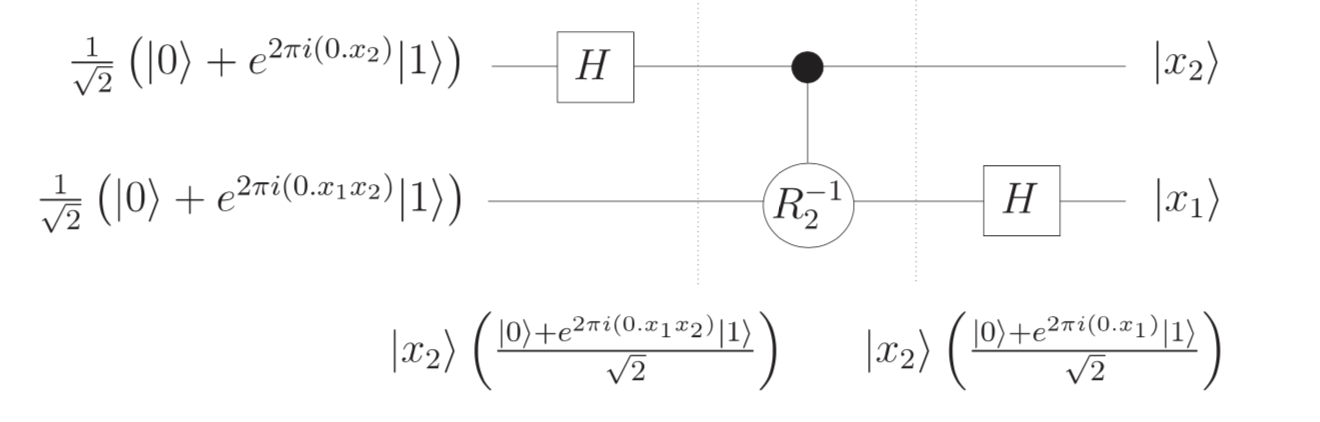
\includegraphics[height=3.5cm]{phase-estimation.png}
\end{frame}
\begin{frame}{Phase estimation technicalities}
This analysis is really incomplete:
\begin{itemize}
    \item We only saw the action $\omega = 0.x_1 x_2$. What if $\omega$ is actually like $2/3$, and cannot be written as $x/2^n$? \pause 
    
    \item Circuit gets more and more complicated for more qubits, but follows the same idea of `pulling' then repeatedly eliminating.
\end{itemize}
\end{frame}
\begin{frame}{Phase estimation backwards: QFT}
    When $\omega \approx 0.x_1 x_2, \ldots x_n$, phase estimation now gives us
    $$
    \frac{1}{\sqrt{2}^n} \sum_{i = 0}^{2^n - 1} e^{2 \pi i \omega y} \ket{y} \mapsto \ket{x_1 x_2 \ldots x_n}$$
    With high probability. \pause
    
    If we just reverse the circuit, we get
    
    $$
     \ket{x_1 x_2 \ldots x_n}  \mapsto \frac{1}{\sqrt{2}^n} \sum_{i = 0}^{2^n - 1} e^{2 \pi i \omega y} \ket{y}
     $$
     
     \pause This replicates the behavior of the discrete fourier transform in a quantum implementation, hence QFT. Phase estimation is called ``$\textsc{QFT}^{-1}$''.
\end{frame}
\section{Shor's Algorithm}
\begin{frame}{Back to factoring}
    \textsc{Factor}
    
    \textbf{Input}: $N = pq$
    
    \textbf{Output}: A factor of $N$, which is either $p$ or $q$. \pause 
    
     \ \\
     \ \\
    
    It turns out this reduces (probabilistically) to a problem called \textsc{Order-find} (if we have a fast algorithm for \textsc{Order-find}, we can use it as a black box to implement \textsc{Factor}) \pause
    
    \ \\
    
    The idea of reductions is very common in computer science, we write $\textsc{Factor} \to \textsc{Order-find}$
\end{frame}
\begin{frame}{Order finding}
    \textsc{Order-find}
    
    \textbf{Input}: $a, N$ with $\text{gcd}(a, N) = 1$.
    
    \textbf{Output}: Minimum $r$ such that $a^{r} = 1 \ (\text{mod } N)$
    
    \pause
    
    \ \\
    \ \\
    
    How come $\textsc{Factor} \to \textsc{Order-find}$?
    
\end{frame}
\begin{frame}{$\textsc{Factor} \to \textsc{Order-find}$?}
    We can pick elements $a \in \{ 0, \ldots N - 1 \}$ randomly. \pause
    
    Checking that $\text{gcd}(a, N) = 1$ is really quick to do classically (Euclid GCD algorithm). \pause
    
    If the order of $a$ is even, then we've lucked out! \pause
    
    $$ a^{r} \equiv 1 \ (\text{mod } N)$$
     $$ (a^{r/2})^2 -1 \equiv 0 \ (\text{mod } N)$$
     $$ (a^{r/2} + 1) (a^{r/2} - 1) \equiv 0 \ (\text{mod } N)$$ \pause
     
    We've just factorized $N$! $a^{r/2} + 1$ and $a^{r/2} - 1$ are almost always nontrivial (meaning not $1$ and $N$) factors.
    
\end{frame}

\begin{frame}{$\textsc{Order-find} \to \textsc{Eigenvalue-estimate}$}

    How can we get $r$, the order, from a quantum algorithm? \pause
    
    Consider $$U_a \colon \ket{s} \mapsto \ket{sa} \ (\text{mod } N)$$ \pause 
    
    $$U_a^r \colon \ket{s} \mapsto \ket{sa^r} \ (\text{mod } N) = \ket{s} $$ \pause
    
    So $U_a^r = I$!
    
    This means its eigenvalues are all $r$th roots of unity, i.e. complex numbers of the form
    
    $$ e^{2 \pi i k/r}, k \in \{0, \ldots, r - 1 \}$$
 
\end{frame}

\begin{frame}{$\textsc{Order-find} \to \textsc{Eigenvalue-estimate}$}
    
    For an eigenvector of $U_a$, $\ket{\psi}$
    
    $$U_a \ket{\psi} = e^{2 \pi i k/r } \ket{\psi}$$ \pause
    
    Modulo some details ($k$, $\psi$), we already have a way to estimate $\omega = k/r$ from phases!! 
 
\end{frame}
\begin{frame}{Eigenvalue estimation}

    \textsc{Eigenvalue-estimate}
    
    \textbf{Input}: A unitary operator $U$ implemented in quantum gates, and an eigenvector $\ket{\psi}$
    
    \textbf{Output}: $\omega$ such that $U \ket{\psi} = e^{2 \pi i \omega} \ket{\psi}$ \pause
    
    (as before, estimated as $\omega = \frac{x}{2^n}$ with $x \in \{ 0, \ldots, 2^n - 1 \}$
    
    \pause
    
    \ \\
    \ \\
    
    Idea: Apply $U$ repeatedly, so we get a quantum state where we can estimate $\omega$ from our phase estimation algorithm
 
\end{frame}
\begin{frame}{Eigenvalue estimation implementation}
    $U \ket{\psi} = e^{2 \pi i 0.x_1 \ldots x_n} \ket{\psi}$ \pause
    
    \  \\
    
    $U^2 \ket{\psi} = (e^{2 \pi i 0.x_1 \ldots x_n})^2 \ket{\psi} = e^{2 \pi i x_1.x_2 \ldots x_{n-1}} \ket{\psi} = e^{2 \pi i 0.x_2 \ldots x_{n-1}} \ket{\psi}$ \pause
    
    \ \\
    
    $U^{2^j} \ket{\psi} = e^{2 \pi i 0.x_j \ldots x_{n-j}} \ket{\psi}$ \pause
    
    \ \\
    \ \\
    So we can use c-$U^{2^j}$ to get the individual qu-bits in the state we want for eigenvalue estimation.
    
\end{frame}
\begin{frame}{Eigenvalue estimation implementation}
    So here is our way to `set up' the states for estimation:
    \centering 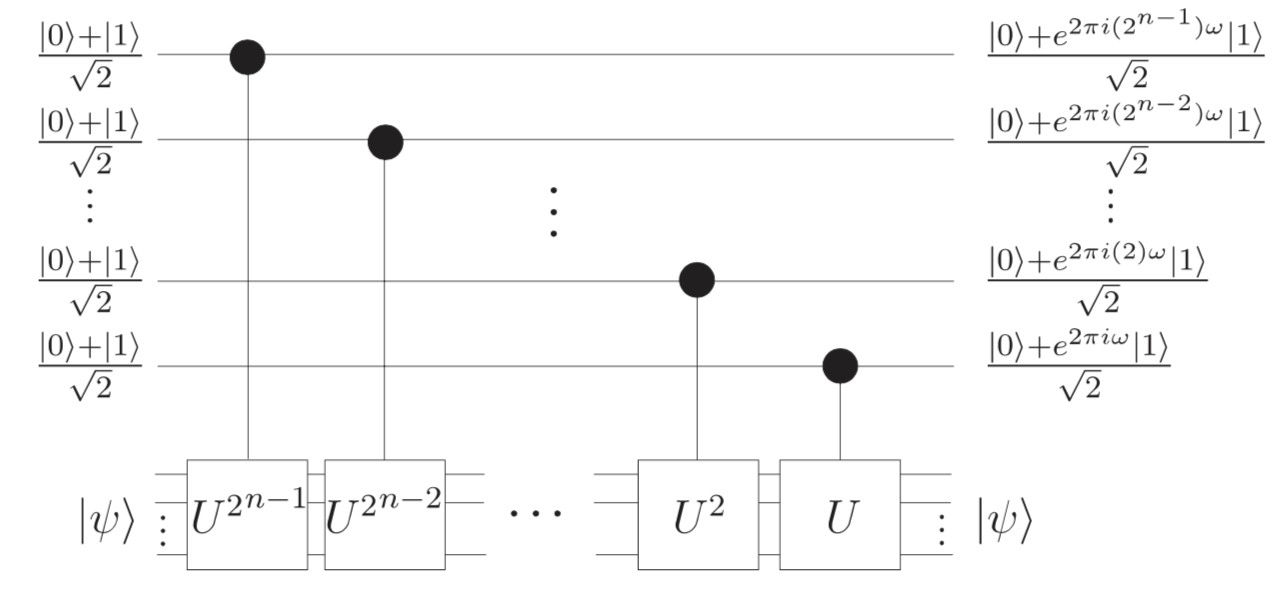
\includegraphics[height=4cm]{eigenvalue-estimation.png}
\end{frame}
\begin{frame}{Eigenvalue estimation implementation}
    It turns out \textsc{QFT} sets up 0 states to $\frac{\ket{0} + \ket{1}}{2}$, so here is our entire diagram (including actually doing phase estimation):
    \centering 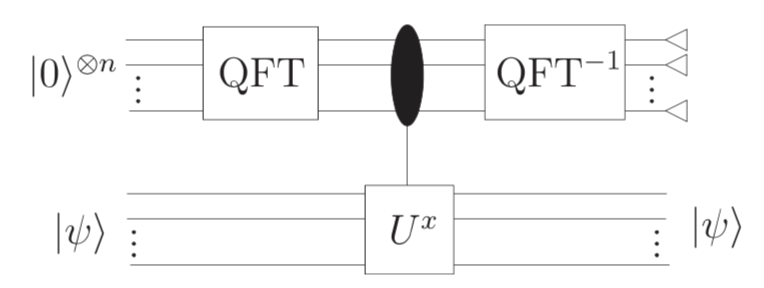
\includegraphics[height=3.5cm]{eigenvalue-estimation-full.png}
\end{frame}

\begin{frame}{Shor's `entire' algorithm}
    We have talked about a way to implement Shor's algorithm (ignoring crucial details like time complexity and correctness):
    
    $$\textsc{Factor} \to \textsc{Order-find} \to$$
    $$\textsc{Eigenvalue-estimate} \to \textsc{Phase-estimate} $$
\end{frame}
\begin{frame}{Implications}
    Factoring numbers quickly breaks security assumptions of RSA. \pause
    
    \ \\
    
    This isn't a huge deal yet. The largest number factored with Shor's algorithm is 21, RSA numbers are on the order of $2^{1024}$. \pause
    
    \ \\
    
    But be careful what you tell people about in 20 years.
    
\end{frame}
\begin{frame}{End}
    Thank you!
    
    \ \\
    \ \\
    \ \\
    Diagrams and much of material from `An Introduction to Quantum Computing', Kaye, Laflamme, Mosca
\end{frame}
\end{document}
